\documentclass[a4paper,11pt]{article}

\usepackage{a4wide}
\usepackage{hyperref}
\usepackage{amsmath,bm,cancel}
\usepackage{tikz}

\newcommand{\td}{\mathrm{d}}
\newcommand{\te}{\mathrm{e}}
\newcommand{\ti}{\mathrm{i}}
\newcommand{\sinc}{\mathrm{sinc}}
\newcommand{\sign}{\mathrm{sign}}
\newcommand{\atan}{\mathrm{atan}}

\title {Analytical integrals of kernels}

\begin{document}

\maketitle

\tableofcontents

\section{Derivatives of kernels depending on the source-receiver distance}

In lots of useful cases (homogeneous and isotropic media) the kernel is distance-dependent: $K({\bf x}, {\bf y}) = G(|{\bf y} - {\bf x}|)$.
In these cases the kernel's normal derivatives can be expressed in a unified way.

Derivatives of the distance vector are given by the following formulas
%
\begin{align}
	r &= |{\bf r}| \\
	r'_i &= \frac{r_i}{r} \\
	r''_{ij} &= \frac{1}{r} \left( \delta_{ij} - r'_i r'_j \right) \\
	r'''_{ijk} &= -\frac{1}{r^2} \left(
		\delta_{ij} r'_k + \delta_{jk} r'_i + \delta_{ki} r'_j - 3 r'_i r'_j r'_k
	\right)
\end{align}

Derivatives of the kernel depending on the distance are formulated as
%
\begin{align}
	G'_i &= G'_r r'_i \\
	G''_{ij} &= \left(G''_r - \frac{G'_r}{r} \right) r'_i r'_j +  \frac{G'_r}{r} \delta_{ij} \\
	G'''_{ijk} &=
	\left(G'''_r -\frac{3}{r} \left(G''_r  - \frac{G'_r}{r} \right) \right) r'_i r'_j r'_k
	+  \frac{1}{r} \left( G''_r  - \frac{G'_r}{r} \right)\left(
	   r'_j \delta_{ki}
	+  r'_i \delta_{jk}
	+  r'_k \delta_{ij}
	\right)
\end{align}


\section{Analytical integrals of the 2D Laplace kernel}

This section describes the analytical formulas used to integrate the kernel of the Laplace equation in two dimensions.

\subsection{Kernel expressions and derivatives}

The kernel and its derivatives are given as
%
\begin{align}
	G(r)
	&= -\frac{\ln r}{2\pi} \\
	G'_{i}
	&= -\frac{1}{2\pi r} \frac{r_i}{r}
	\label{eq:laplace_gradient}
	\\
	G''_{ij}
	&= \frac{-1}{2\pi r^2}\left( \delta_{ij} - 2\frac{r_j}{r} \frac{r_i}{r}\right)
	\label{eq:laplace_second_derivative}
	\\
	G'''_{ijk}
	&= \frac{1}{\pi r^3} \left(
	\delta_{ij} \frac{r_k}{r}
	+ \delta_{jk} \frac{r_i}{r}
	+ \delta_{ki} \frac{r_j}{r}
	-4 \frac{r_i}{r} \frac{r_j}{r} \frac{r_k}{r}
	\right)
	\label{eq:laplace_third_derivative}
\end{align}

The normal derivative w.r.t $n_y$ is computed as $G'_i n_{yi}$, while the normal derivative w.r.t. $n_x$ is computed as $-G'_i n_{xi}$:
%
\begin{align}
	\frac{\partial G}{\partial n_y} 
	&= n_{yi} G'_i
	&&
	%= -\frac{1}{2\pi r} \frac{n_{yi} r_i}{r}
	= -\frac{1}{2\pi r} r'_{n_y}
	\\
	\frac{\partial^2 G}{\partial n_x \partial n_y}
	&= -n_{xi} n_{yj} G''_{ij}
	&&
	%= \frac{1}{2\pi r^2}\left( n_{xi} n_{yi} - 2\frac{r_j n_{yj}}{r} \frac{r_i n_{xi}}{r}\right)
	= \frac{1}{2\pi r^2}\left( n_{xi} n_{yi} + 2 r'_{n_x} r'_{n_y}\right)
	\\
	\frac{\partial^2 G}{\partial n_x^2}
	&= n_{xi} n_{xj} G''_{ij}
	&&
	%= \frac{1}{2\pi r^2}\left( -1 + 2 \left(\frac{r_j n_{xj}}{r}\right)^2 \right)
	= \frac{1}{2\pi r^2}\left( -1 + 2 \left(r'_{n_x}\right)^2 \right)
	\\
	\frac{\partial^3 G}{\partial n_x^2 \partial n_y}
	&= n_{xi} n_{xj} n_{yk} G'''_{ijk}
	&&
	= \frac{1}{\pi r^3} 
	 \left(
	r'_{n_y}
	- 2 r'_{n_x} \left(n_{xk} n_{yk}\right)
	-4 \left(r'_{n_x}\right)^2 r'_{n_y}
	\right)
\end{align}

\subsection{Collocation}

The following parts describe the case of collocation where ${\bf x}={\bf x}_0$ is a fixed location and integration is performed with respect to the variable ${\bf y}$. In general, the integrals are written in the form
%
\begin{equation}
\int_S K({\bf y}, {\bf x}_0) N({\bf y}) \td S_y
\end{equation}
%
where $K$ denotes one of the kernels introduced above, and $N({\bf y})$ denotes (polynomial) weighting functions over the element.

\subsubsection{Regular integrals}

\begin{figure}
\center
\begin{tikzpicture}[scale=1]
\small
\draw [thin, ->] (2,1) -- (3,.5) node [right] {$\xi$};
\draw [thin, ->] (2,1) -- (2.5,2) node [left] {$\eta$};
\path [draw, fill] (3,3) circle(.05) node [right] {${\bf x}_0$};
\path [draw, very thick, fill] (4,0) circle(.05) node [below] {${\bf y}_2$} -- (4.5,-.25) circle(.05) node [below] {${\bf y}$} -- (6,-1) circle(.05) node [below] {${\bf y}_1$};
\path [draw, thick, ->] (5,-.5) -- (5.5,.5) node [above] {${\bf n}$};
\end{tikzpicture}
\caption{Coordinate transform for the definition of the regular integrals over the straight line element}
\label{fig:regular_local}
\end{figure}

In order to define the regular integrals in a convenient way local coordinates are introduced, as shown in Fig.~\ref{fig:regular_local}:
%
\begin{align}
\xi &= ({\bf y} - {\bf x}_0) \cdot {\bf t} \qquad {\bf t} = \frac{{\bf y}_1 - {\bf y}_2}{|{\bf y}_1 - {\bf y}_2|} \nonumber \\
\eta &= ({\bf x}_0 - {\bf y}) \cdot {\bf n}
\end{align}
%
The straight line element lies in the $\eta = 0$ line. The nodal locations ${\bf y}_1$ and ${\bf y}_2$ correspond with the local coordinates $\xi_1$ and $\xi_2$, respectively, and due to the proper selection of the normal's direction, $\xi_1 = \xi_2 + d$ where $d$ is the element length. The origin of the local system is the image of ${\bf x}_0$ on the element's line.

The regularity of the integrals is ensured if $\eta \ne 0$ or $\sign \xi_1 = \sign \xi_2$


\paragraph{SLP kernel}

The regular integral of the single layer potential kernel can be now written in the general form
%
\begin{align}
I &= \frac{-1}{2\pi} \int_{\xi_2}^{\xi_1} \ln\left(\sqrt{\xi^2+\eta^2}\right) \left(a_0 + a_1 \xi + a_2 \xi^2\right) \td \xi \\
 &= \frac{1}{2\pi} \left[
\left(\frac{1}{9} - \frac{\ln \rho}{3}\right) a_2 \xi^3
+ \frac{a_1}{2} \left(\frac{\xi^2}{2}
- \rho^2 \ln \rho\right)
- a_0 \xi \ln \rho
+ \left(\frac{a_2 \eta^2}{3} - a_0 \right) \left(\eta \atan\frac{\xi}{\eta} - \xi\right)
\right]_{\xi_2}^{\xi_1} \nonumber
\end{align}
%
where $\rho = r = \sqrt{\xi^2+\eta^2}$.

\paragraph{DLP kernel}

For the case of the double layer potential kernel, the integral is transformed as
%
\begin{equation}
I = \frac{-1}{2\pi} \int_{\xi_2}^{\xi_1} \frac{-\eta \left(a_0 + a_1 \xi + a_2 \xi^2 \right)}{\xi^2+\eta^2}\td \xi
= \frac{1}{2\pi} \left[
\left( a_0 - a_2 \eta^2\right) \atan \frac{\xi}{\eta} + \left(a_2 \xi + a_1 \ln r\right) \eta
\right]_{\xi_2}^{\xi_1}
\end{equation}

\paragraph{HSP kernel}

For the case of the HSP kernel, let $n_{\xi}$ and $n_{\eta}$ denote the normal at $x_0$ in the local frame of reference. In this case the integral is expressed as
%
\begin{equation}
I
= \int_{\xi_2}^{\xi_1} G''_{n_x n_y} \td \xi
= -\frac{1}{2\pi} \left[ \frac{ \eta n_{\xi} + \xi n_{\eta} }{\rho^2} \right]_{\xi_2}^{\xi_1}
\end{equation}

\subsubsection{Singular integrals}

\paragraph{General SLP}

\begin{equation}
	I = \int_S G(r) N(y) \td S
\end{equation}
%
In the reference domain
%
\begin{equation}
	I = \int_a^b G(\rho) N(\rho) J(\rho) \td \rho
\end{equation}
%
where $\rho = \eta - \xi$ denotes the signed distance from the singular point in the reference domain.

Taylor expansion of the distance
%
\begin{equation}
	{\bf r} = \rho {\bf r}_1 + \frac{\rho^2}{2} {\bf r}_2 + O(\rho^3)
\end{equation}
%
Taylor expansion of the scalar squared distance:
%
\begin{align}
	r^2 &= \rho^2 r_1^2 (1 + \rho A + O(\rho^2)), \qquad A = \frac{{\bf r}_1 {\bf r}_2}{r_1^2} \\
	r &= |\rho| r_1 \left(1 + \frac{\rho A}{2} + O(\rho^2)\right)
\end{align}
%
Taylor expansion of the Green's function around the singular point
%
\begin{equation}
	G(r) = -\frac{1}{2\pi} \left(
		\log (|\rho| r_1) + \rho \frac{A}{2} + O(\rho^2)
		\right)
\end{equation}
%
The singular part of the integral is
%
\begin{equation}
	F_0 = -\frac{1}{2\pi} \log \left(|\rho| r_1\right) N_0 J_0
\end{equation}
%
and its integral over the element is computed as
%
\begin{equation}
	\int_{a}^b F_0 \td\rho
	= \frac{-N_0 J_0}{2\pi} \left(|b|(\log(|b| J_0) - 1) + |a|(\log(|a| J_0) - 1) \right)
\end{equation}

\paragraph{Constant line SLP}

\begin{align}
\int_{S} G({\bf y}, {\bf x}) \td y
& = \frac{-1}{2\pi}\lim_{\epsilon \to 0}
\left( \int_{-d_1}^{-\epsilon} \ln |y| \td y + \int_{\epsilon}^{d_2}  \ln |y| \td y \right) \nonumber \\
& = \frac{-1}{2\pi}\lim_{\epsilon \to 0}
\left( \int_{\epsilon}^{d_1} \ln y \td y + \int_{\epsilon}^{d_2}  \ln y \td y \right) \nonumber \\
&=
\frac{d_1(1-\ln d_1) + d_2(1-\ln d_2)}{2\pi}
\end{align}

\paragraph{Constant line DLP}

\begin{equation}
\int_{S} G'_{n_y}({\bf y}, {\bf x}) \td y = 0
\end{equation}
%
as the element normal is perpendicular to the distance ${\bf y}-{\bf x}$.

\paragraph{Constant line HSP}

Finite part integral with general shape function $N(y)$
%
\begin{align}
	I = \int_S G''_{n_x n_y}({\bf y}, {\bf x}) N({\bf y}) \td y
	&= \frac{1}{2\pi} \int_S \frac{1}{(y-x)^2} N(y) \td y \\
	&= \frac{1}{2\pi} \int_\Sigma \frac{1}{J^2 (\eta-\xi)^2} N(\eta) J \td \eta \\
	&= \frac{1}{2\pi J} \left(
		\int_a^{\xi-\epsilon} \frac{1}{(\eta-\xi)^2} N(\eta) \td \eta
		+ \int_{\xi+\epsilon}^{b} \frac{1}{(\eta-\xi)^2} N(\eta) \td \eta
	\right)
\end{align}

The shape function is written with its Taylor series around the singular point
%
\begin{equation}
	N(\eta) = N(\xi) + N'(\xi) (\eta-\xi) + \sum_{k=2}^{\infty} \frac{N^{(k)}(\xi)}{k!}(\eta-\xi)^k
\end{equation}

Substitution yields

\begin{equation}
	I = \frac{N(\xi)}{2\pi J} \left(
		\cancel{\frac{1}{2\epsilon}} + \left[ \frac{-1}{\eta-\xi} \right]_{a}^{b} 
	\right)
	+
	\frac{N'(\xi)}{2\pi J} \log \frac{|b-\xi|}{|a-\xi|}
	+ \sum_{k=2}^{\infty} \frac{N^{(k)}(\xi)}{2\pi J k! (k-1)}
		\left[ (\eta-\xi)^{k-1} \right]_{a}^{b} 
\end{equation}

\paragraph{General element HSP}

General approach for curved elements
%
\begin{align}
	I = \int_S G''_{n_x n_y}({\bf y}, {\bf x}) N({\bf y}) \td y
	= \int_a^b G''_{n_x n_y}(\rho) N(\rho) J(\rho) \td \rho
\end{align}
%
where $\rho = \eta - \xi$ denotes the signed distance from the singular point in the reference domain.

In order evaluate the singular part of the integral analytically, the following Taylor series expansions are introduced:
\begin{align}
	{\bf r}(\rho) &= {\bf y} - {\bf x} = \rho {\bf r_1} + \frac{\rho^2}{2} {\bf r}_2 + O(\rho^3) \\
	{\bf d}(\rho) &= \frac{\td {\bf r}(\rho)}{\td \rho} = {\bf r_1} + \rho {\bf r}_2 + O(\rho^2)\\
	{\bf J}(\rho) &= {\bf T} {\bf d}(\rho) = {\bf J}_0 + \rho {\bf J}_1 + O(\rho^2) \\
	r^2 &= \rho^2 r_1^2 \left( 1 + A \rho + O(\rho^2) \right)
	,\quad A = \frac{{\bf r}_1 {\bf r}_2}{r_1^2} \\
	\frac{1}{r^2(\rho)} &\approx \frac{1 - A \rho + O(\rho^2)}{\rho^2 r_1^2}
\end{align}

The Green's function $G''$, multiplied with the Jacobian $J$ in the local frame of reference is approximated as (replacing $n_y$ by $J$)
%
\begin{equation}
	G''(\rho) J(\rho)
	= \frac{1}{2\pi r^2(\rho)} \left( {\bf n}_x {\bf J}(\rho) - 2 \frac{{\bf r}(\rho) {\bf n}_x}{r(\rho)} \frac{{\bf r}(\rho) {\bf J}(\rho)}{r(\rho)}\right)
\end{equation}
%
The second term in the bracketed part is $O(\rho^2)$.
The first order Taylor series approximation of the first term is
%
\begin{equation}
	G''(\rho) J(\rho) \approx \frac{1 - A \rho}{2\pi \rho^2 r_1^2} {\bf n}_x \left({\bf J}_0 + \rho {\bf J}_1\right) 
\end{equation}
%
Exploiting that ${\bf n}_x \left({\bf J}_0 + \rho {\bf J}_1\right) = J_0 (1 + \rho A)$, and $r_1^2 = J_0^2$, the final first order Taylor series expansion of the kernel is
%
\begin{equation}
	G''(\rho) J(\rho) \approx \frac{1}{2\pi \rho^2 J_0}
\end{equation}
%
and the singular part of the integrand is
%
\begin{equation}
	G''(\rho) N(\rho) J(\rho) \approx \frac{1}{2\pi J_0} \left( \frac{N_0}{\rho^2} +  \frac{N_1}{\rho} \right)
\end{equation}


\subsection{Galerkin}

\subsubsection{Face match}

\paragraph{Constant line SLP}

\begin{equation}
\int_{0}^{d}
\lim_{\epsilon \to 0}
\left(
\int_{0}^{x-\epsilon} G(x-y) \td y
+
\int_{x+\epsilon}^{d} G(x-y) \td y
\right)
\td x
=
d^2\frac{3-2\ln d}{4\pi}
\end{equation}

\paragraph{Linear line SLP}

\begin{equation}
\int_{0}^{d} N_i(x) \int_{0}^{d} G(x-y) N_j(y) \td y \td x
=
\frac{d^2}{32\pi} \begin{bmatrix}
7-4 \ln d & 5 - 4 \ln d \\
5-4 \ln d & 7 - 4 \ln d
\end{bmatrix}
\end{equation}

\subsubsection{Edge match}

The local coordinate system used for the calculation of edge-match type singular integrals is shown in Fig.~\ref{fig:local_galerkin_edge}. The lengths of the elements are denoted with $d_1$ and $d_2$, and the second element defines the direction of the normal vector. The angle between the two elements is denoted by $\phi$.

\begin{figure}
\center
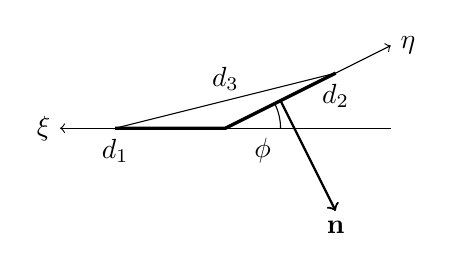
\begin{tikzpicture}[scale=.7]
\path [draw, ->] (3,0) -- (-3,0) node [left] {$\xi$};
\path [draw, ->] (0,0) -- (3,1.5) node [right] {$\eta$};
\path [draw] (-2,0) --  node [above] {$d_3$} (2,1);
\path [draw, very thick] (-2,0) node [below] {$d_1$} -- (0,0) -- (2,1) node [below] {$d_2$};
\path [draw, thick, ->] (1,.5) -- (2,-1.5) node [below] {${\bf n}$};
\draw [domain=0:26.5] plot ({cos(\x)}, {sin(\x)});
\path (1,0) node [below left] {$\phi$};
\end{tikzpicture}
\caption{Local coordinates for the definition of Galerkin edge-match singular integrals}
\label{fig:local_galerkin_edge}
\end{figure}

\paragraph{Constant line SLP}

\begin{multline}
\int_{S_{x}} \int_{S_{y}} G(r) \td S_y \td S_x =
\int_{0}^{d_1} \int_{0}^{d_2}
\frac{-1}{2\pi}\ln \sqrt{(\xi+\eta \cos\phi)^2 + (\eta\sin\phi)^2}
\td \eta \td \xi \\
=
\frac{1}{4 \pi}
\left[
d_1 d_2 \left(3 - 2 \ln d_3 \right)
+ \cos\phi \left(d_1^2 \ln \frac{d_1}{d_3} + d_2^2 \ln \frac{d_2}{d_3}\right)
- \sin\phi \left(d_1^2 q\left(\frac{d_2}{d_1}, \phi\right) + d_2^2 q\left(\frac{d_1}{d_2}, \phi\right)\right)
\right]
\end{multline}
%
where
%
\begin{equation}
q(a, \phi) = \atan\left(\frac{a}{\sin\phi} + \cot\phi\right) - \atan\left(\cot\phi\right)
\end{equation}

\paragraph{Constant line DLP}

\begin{align}
\int_{S_{x}} \int_{S_{y}} G'(r) r'_{n_{y}} \td S_y \td S_x
&=
\frac{-1}{2\pi}\int_{0}^{d_1} \int_{0}^{d_2}
\frac{\xi\sin\phi}{(\xi+\eta \cos\phi)^2 + (\eta\sin\phi)^2}
\td \eta \td \xi \nonumber \\
&=
\frac{1}{2\pi}\left[
	d_2 \cos\phi q\left(\frac{d_1}{d_2}, \phi\right)
	- d_1 q\left(\frac{d_2}{d_1}, \phi\right)
	+ d_2 \sin\phi \ln \frac{d_2}{d_3}
\right]
\end{align}



\section {Analytical integrals of the 2D Helmholtz kernel}

\subsection{Introduction}

The kernel is defined as
%
\begin{equation}
	G({\bf y}, {\bf x}) = \frac{-\ti}{4} H_0^{(2)}(kr), \quad r = |{\bf y} - {\bf x}|
\end{equation}
%
where ${\bf x}$ is the source point. The kernel exhibits a weak (integrable) singularity when $r \to 0$.

The Hankel function may be written as
%
\begin{equation}
	H_0^{(2)}(z) = J_0(z) - \ti Y_0(z)
\end{equation}
%
and the small argument series expansion of the involved Bessel functions around $z=0$ are
%
\begin{align}
	J_0(z) &= \sum_{n=0}^{\infty} (-1)^n \frac{\left(\frac{z}{2}\right)^{2n}}{\left(n!\right)^2} \\
	Y_0(z) &= \frac{2}{\pi}
	\sum_{n=0}^{\infty} (-1)^n \left(\log \frac{z}{2} + \gamma - C_n \right) \frac{\left(\frac{z}{2}\right)^{2n}}{\left(n!\right)^2}
\end{align}
%
where $\gamma$ denotes Euler's constant and $C_n$ denotes the harmonic sum
%
\begin{equation}
	C_0 = 0, C_n = C_{n-1} + \frac{1}{n}
\end{equation}

The kernel's gradient is expressed as
%
\begin{equation}
	G'_i = -\frac{\ti k}{4} H_0^{,(2)}(kr) r'_i
	= \frac{\ti k}{4} H_1^{(2)}(kr) \frac{r_i}{r}
\end{equation}


The kernel's second derivative tensor is expressed as
%
\begin{multline}
	G''_{ij}
	= -\frac{\ti k}{4} \left( H_0^{,(2)}(kr) r'_j \right)'_i
	= -\frac{\ti k}{4} \left( H_0^{,,(2)}(kr) k r'_i r'_j + H_0^{,(2)}(kr) \left(\frac{\delta_{ij}}{r} - \frac{r_i r_j}{r^3}\right)\right) \\
	= -\frac{\ti k}{4} \left( \frac{1}{2} \left(H_2(kr) - H_0(kr) \right) k \frac{r_i r_j}{r^2} - \frac{H_1^{(2)}(kr)}{r} \left(\delta_{ij} - \frac{r_i r_j}{r^2}\right)\right) \\
	= \frac{\ti k^2}{4} \left( \left( \frac{1}{2} H_0(kr) - \frac{H_1^{(2)}(kr)}{kr} -\frac{1}{2} H_2(kr) \right) \frac{r_i r_j}{r^2} + \frac{H_1^{(2)}(kr)}{kr} \delta_{ij} \right)
\end{multline}

As a consequence, the second normal derivative is expressed as

\begin{equation}
	G''_{n_{x} n_{y}}
	= \frac{\ti k^2}{4} \left( \left( \frac{1}{2} H_0(kr) - \frac{H_1^{(2)}(kr)}{kr} -\frac{1}{2} H_2(kr) \right)
	r'_{nx} r'_{ny}
	- \frac{H_1^{(2)}(kr)}{kr} n_{xi} n_{yi}\right)
\end{equation}


\subsection{Collocation}

\paragraph{Constant line SLP}

The integral to evaluate can be simplified to the form
%
\begin{equation}
I = \frac{-\ti}{4} \int_{-R}^R  H_0^{(2)}(kr)  \td y
\end{equation}
%
where $R$ denotes the element's half length.

From the above series expansions, the integral $I$ may be expressed in terms of the following integral elements ($D = 2R$):
%
\begin{align}
\int_{-R}^R
\left(\frac{kr}{2}\right)^{2n} \td y
= D \left( \frac{kR}{2} \right)^{2n} F_n \\
\int_{-R}^R
\log \frac{kr}{2} \cdot \left(\frac{kr}{2}\right)^{2n} \td y
= D \left(\frac{kR}{2}\right)^{2 n} G_n
\end{align}
%
where
%
\begin{align}
F_n &= \frac{1}{2n+1} \\
G_n &= \frac{\log\frac{kR}{2}} {2 n + 1} - \frac{1}{(2 n + 1)^2}
\end{align}


\subsection{Galerkin}

\subsubsection{Face match}

\paragraph{Constant line SLP}

The integral to evaluate can be simplified to the form
%
\begin{equation}
I = \frac{-\ti}{4} \int_{-R}^{R} \int_{-R}^R  H_0^{(2)}(k|y-x|)  \td y \td x
\end{equation}
%
where $R$ denotes the element's half length.

From the above series expansions, the integral $I$ may be expressed in terms of the following integral elements ($r=|y-x|$, $D = 2R$):
%
\begin{align}
\int_{-R}^{R} \int_{-R}^R  \left(\frac{kr}{2}\right)^{2n}  \td y \td x
= D^2 \cdot (kR)^{2n} F_n
\\
\int_{-R}^{R} \int_{-R}^R  \log \frac{kr}{2} \cdot \left(\frac{kr}{2}\right)^{2n}  \td y \td x
= D^2 \cdot (kR)^{2n} G_n
\end{align}
%
where
%
\begin{align}
F_n &= \frac{1}{(n+1)(2n+1)}
\\
G_n &= \begin{cases}
\log kR - \frac{2}{3} & n = 0 \\
\frac{\log kR}{(n+1)(2n+1)} - \frac{4n+3}{2(n+1)^2(2n+1)^2}& n > 0
\end{cases}
\end{align}

As a result, the total integral is expressed as
%
\begin{equation}
I = -\ti R^2
\sum_{n=0}^{\infty} (-1)^n \frac{(kR)^{2n}}{\left(n!\right)^2}
\left(
F_n
- \frac{2 \ti}{\pi}
\left(G_n + \left(\gamma - C_n \right) F_n \right)
\right)
\end{equation}


\section{Analytical integrals of the 3D Laplace kernel}

The kernel is defined as
%
\begin{equation}
	G({\bf r}) = \frac{1}{4\pi|{\bf r}|} = -\frac{1}{4\pi r}
\end{equation}

\subsection{Derivatives}

The kernel's first, second and third derivatives can be formulated as
%
\begin{align}
	G'_{i}
	&= -\frac{1}{4\pi r^2} \frac{r_i}{r}
	\label{eq:laplace_3d_gradient}
	% \\
	% G''_{ij}
	% &= \frac{-1}{2\pi r^2}\left( \delta_{ij} - 2\frac{r_j}{r} \frac{r_i}{r}\right)
	% \label{eq:laplace_3d_second_derivative}
	% \\
	% G'''_{ijk}
	% &= \frac{1}{\pi r^3} \left(
	% \delta_{ij} \frac{r_k}{r}
	% + \delta_{jk} \frac{r_i}{r}
	% + \delta_{ki} \frac{r_j}{r}
	% -4 \frac{r_i}{r} \frac{r_j}{r} \frac{r_k}{r}
	% \right)
	% \label{eq:laplace_3d_third_derivative}
\end{align}



\subsection{Normal derivatives}


\subsection{Collocation}

For the collocational singular integrals over plane surfaces, the following geometry is used, as shown in Figure \ref{fig:tria_angles}.
The plane polygon is split up into triangles by connecting the collocational point ${\bf x}_0$ with the corners.
The polar coordinates $\rho, \theta$ are defined separately for each triangle, as shown in the figure.

From the law of sines, $R(\theta)$ is expressed as
%
\begin{equation}
	R(\theta) = \frac{R \sin(\alpha)}{\sin(\theta+\alpha)}
\end{equation}


\begin{figure}
	\center
	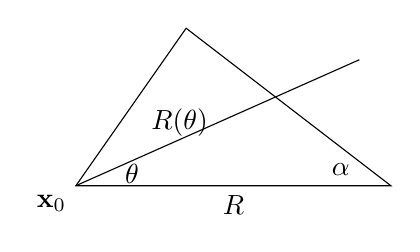
\begin{tikzpicture}[scale=2]
	\path [draw] (0,0) node [anchor = north east] {${\bf x}_0$} -- node [anchor = north] {$R$} (2,0) -- (.7, 1) -- cycle;
	\path [draw] (0,0) -- node [anchor = east] {$R(\theta)$} (1.8,.8);
	\path (.25,-.05) node [anchor = south west] {$\theta$};
	\path (1.8,0) node [anchor = south east] {$\alpha$};
	\end{tikzpicture}
	\caption{The plane polygon is split up into triangles}
	\label{fig:tria_angles}
\end{figure}



\subsubsection{Regular integrals}

\subsubsection{Plane constant SLP}

The collocational singular integral of the SLP kernel with constant shape function is written in polar coordinates as
%
\begin{equation}
\int_0^{\theta_0} \int_0^{R(\theta)} \frac{r \td r \td \theta}{4\pi r}
=
\frac{1}{4\pi}\int_0^{\theta_0} R(\theta) \td \theta
=
\frac{R \sin(\alpha)}{4\pi}\int_0^{\theta_0} \frac{1}{\sin(\theta+\alpha)} \td \theta
\end{equation}

%
using the identity
%
\begin{equation}
\int \frac{\td x}{\sin x} = \log \tan (x/2)
\end{equation}
%
the integral can be expressed (by summing for $n$ triangles) as follows:
%
\begin{equation}
I = \frac{1}{4\pi} \sum_{i = 1}^n
R_i \sin\alpha_i \left[ \log \left( \frac{\tan\left(\frac{\phi_i+\alpha_i}{2}\right)}{\tan\left(\frac{\alpha_i}{2}\right)}\right)\right]
\end{equation}

\subsubsection{Plane constant HSP}

\begin{equation}
	\int \frac{1}{4\pi r^3} \td S
	= \frac{1}{4\pi}\int \int_{0}^{R(\theta)} \frac{r \td r}{r^3} \td \theta
	= \frac{-1}{4\pi}\int \frac{1}{R(\theta)} \td \theta
	= \frac{\cos(\theta+\alpha)}{4\pi R \sin(\alpha)}
\end{equation}

\end{document}

